\documentclass[12pt,a4paper]{article}

\usepackage{url}
\usepackage{appendix}
\usepackage[british]{babel}
\usepackage{amsmath}
\usepackage{hyperref}
\usepackage{graphicx}
\numberwithin{equation}{section}
\numberwithin{figure}{section}
\numberwithin{table}{section}

\usepackage[round]{natbib}
\bibliographystyle{natbib}
\def\bibsection{\section*{References}}

% Wrap around which gives all figures included the [H] command, or places it "here". This can be tedious to code in Rmarkdown.
\usepackage{float}
\let\origfigure\figure
\let\endorigfigure\endfigure
\renewenvironment{figure}[1][2] {
    \expandafter\origfigure\expandafter[H]
} {
    \endorigfigure
}

\let\origtable\table
\let\endorigtable\endtable
\renewenvironment{table}[1][2] {
    \expandafter\origtable\expandafter[H]
} {
    \endorigtable
}

\def\tightlist{}

\bibpunct[:]{(}{)}{;}{a}{,}{,}

\renewcommand{\baselinestretch}{1.5}

\begin{document}

\begin{titlepage}

\begin{center}
{\Huge \bf How does the latest Prophet forecasting model compare to the ARIMA
model? Evaluation of BTC/ZAR predictability through a Mincer-Zarnowitz
approach}\\
\today\\
Fiona Ganie (GNXFIO001)\\
{\tt GNXFIO001@myuct.ac.za}
\end{center}

\begin{abstract}
The Autoregressive Integrated Moving Average (ARIMA) model is one of the
most widely used time series models that has gained popularity in the
exchange rate market due to its ease of implementation and tractability.
With the evolution of computational power, soft computing techniques
have since been used in exchange rate markets. The ARIMA model has been
used as the standard benchmark model against which these complex methods
have been compared. Although they have produced significantly better
results than the ARIMA model, these models lack interpretability and
building them is a challenging task. Prophet is a sophisticated model
that differs to traditional time series models in that it can be
utilised by non-experts who have little knowledge about the statistical
intricacies involved in the model, however have domain knowledge about
the data generating process. Prophet is also robust to outliers and can
handle missing values in the time series without the need for
interpolation. This paper compares the out-of-sample forecasts of
Prophet and ARIMA over varying forecast horizons, using a
Mincer-Zarnowitz approach for forecast evaluation. A complete dataset of
the prices of Bitcoin/Rand as well as a dataset which has missing prices
and outliers present is used in the analysis. It is found that the ARIMA
model produces the most efficient and unbiased forecasts over all
forecast horizons, and that the ARIMA model is more robust when faced
with missing values and outliers present in the data.
\noindent
Keywords: Prophet, ARIMA, Mincer-Zarnowitz,   Box-Jenkins, Bitcoin.
\end{abstract}
\end{titlepage}

\pagenumbering{arabic}

\section{\texorpdfstring{Introduction
\label{Introduction}}{Introduction }}\label{introduction}

The Autoregressive Integrated Moving Average (ARIMA) model is one of the
most widely used time series models that has attracted attention in
financial market forecasting (Khashei, Bijari, and Ardali 2009).
Although the Random Walk model has typically been applied to foreign
exchange markets and has produced superior results, some researchers
have contended that foreign exchange markets are not efficient and
believe that future prices depend on current and past events
(Abu-Mostafa and Atiya 1996). This has led to the application of the
ARIMA model to exchange rate problems, where it has since gained
popularity due to its ease of implementation and tractability. The ARIMA
model is easy to use and yields good forecasts over short forecast
horizons, however the linearity of the ARIMA model fails to adequately
capture the non-linearity inherent in exchange rate data (Zhang and Hu
1998).

With the evolution of computational power, non-linear, soft computing
techniques have been proposed as a solution. The ARIMA model has been
used as the standard benchmark model against which these more complex
methods have been compared. Although they have produced significantly
better results than the ARIMA model, these models lack interpretability
and building them is a challenging task. The ARIMA model is tractable
and less computationally expensive. It has been used as the building
blocks for more advanced models and has provided the inspiration for
hybrid versions of the model which have been used in exchange rate
forecasting.

In December 2016, Facebook open-sourced their forecasting model Prophet.
Prophet differs to traditional time series model such as the ARIMA, in
that it can produce high quality forecasts in a straightforward way.
Prophet is a sophisticated model that provides informative results,
however is configurable and easy to use. It can be utilised by
non-experts who have little knowledge about the statistical intricacies
involved in the model, however have domain knowledge about the data
generating process. This knowledge can be easily incorporated into the
model through its intuitively adjustable parameters (Taylor and Letham
2017). Furthermore, Prophet is robust to outliers and can handle missing
values in the time series without the need for interpolation (Taylor and
Letham 2017). This allows analysts without knowledge on how to
pre-process the data, to utilise the model without sacrificing
predictive accuracy. If Prophet produces forecasts that are as good as
the ARIMA model, it can be compared to more complex forecasting methods
that are less tractable and flexible.

This paper broadly aims to compare the forecasts produced by the
traditional ARIMA model and Prophet through an evaluation of the
exchange rate between Bitcoin and the Rand (BTC/ZAR), using a
Mincer-Zarnowitz approach of measuring forecast accuracy. More
specifically, this paper aims to:

\begin{enumerate}
\def\labelenumi{\arabic{enumi}.}
\item
  Compare the out-of-sample forecasts of ARIMA and Prophet over varying
  forecast horizons.
\item
  Compare the out-of-sample forecast performance with missing values and
  outliers present in the data.
\end{enumerate}

Section \ref{Background and Theory} will present the key findings from
the major works in which comparisons have been made to the ARIMA model
in exchange rate forecasting, as well as the theory behind the ARIMA and
Prophet model. Section \ref{Data} will provide a brief explanation and
motivation for the dataset used in this paper. Section \ref{Methodology}
will describe the methodology used in selecting the ARIMA and Prophet
models and the Mincer-Zarnowitz approach of measuring forecast accuracy.
The results from applying the ARIMA and Prophet model to the dataset is
presented in Section \ref{Results}. Finally, Section
\textbackslash{}ref\{Discussion and Conclusions discusses the results in
a statistical context.

\section{\texorpdfstring{Background and Theory
\label{Background and Theory}}{Background and Theory }}\label{background-and-theory}

\subsection{Forecasting Exchange Rates with the ARIMA
model}\label{forecasting-exchange-rates-with-the-arima-model}

ARIMA models became highly popular since its introduction by Box and
Jenkins, when it was shown that they could outperform complex
econometric models in a variety of situations (Hibon and Makridakis
1997). The ARIMA model expresses the process \{\(y_t\)\} as a function
of the weighted average of past values of the process and lagged values
of the residuals. The weighted average of the past p values of the
process represents an autoregressive (AR) process of order p.~It feeds
back past values of the process into the current value, inducing
correlation between all lags of the process. The weighted average of the
q lagged residuals represents a moving average (MA) process of order q.
The purpose of mixing the MA process with the AR process is to reduce
the large number of past values required by AR processes and to control
for the autocorrelation which it creates between lagged values of the
process. The combination of the AR(p) and MA(q) process results in a
more parsimonious model, and forms a stationary autoregressive moving
average (ARMA(p,q)) process defined as:

\[ 
    y_t = c + \sum_{i = 1}^{p} \theta_{i} y_{t-i} + \sum_{i = 1}^{q} \phi_{i} e_{t-i}+ e_t \label{eq1} \\ \notag
\] where c is a constant and \{\(e_t\)\} is a white noise process with
zero mean and variance \(\sigma^2\).

The ARIMA(p,d,q) model generalises the ARMA model in that it includes
both stationary and non-stationary processes. The parameter d is the
degree of differencing required to render the process stationary. If d
is equal to zero the process is stationary and equivalent to an ARMA
model, and if d is strictly positive the process requires differencing
to make it stationary. The ARIMA model can be defined succinctly using
the backward shift operator B, which shifts the process back by one unit
of time, and is defined as \(By_t = y_{t-1}\). The ARIMA model has the
form:

\[ 
    (1-\sum_{i = 1}^{p} \theta_{i} B^i)(1-B)^dy_t = c + (1 + \sum_{i = 1}^{q} \phi_{i} B^i)e_t \label{eq2} \\ \notag 
\] where c is a constant and \{\(e_t\)\} is a white noise process with
zero mean and variance \(\sigma^2\).

ARIMA models have commonly been used in financial forecasting and are
popular for observing stock prices and exchange rates due to its power
and statistical properties (C.-S. Lin, Chiu, and Lin 2012). They have
frequently been used as a benchmark to compare new forecasting
techniques that have emerged over time. Kamruzzaman and Sarker (2003)
applied an ARIMA model to forecast the exchange rate between the
Australian dollar and six other currencies, and used the forecast errors
as well as the accuracy of the direction of the forecasts to evaluate
the performance of three Neural Network models. In a similar study,
Khashei, Bijari, and Ardali (2012) compared the predictive capability of
their proposed hybrid model consisting of an ARIMA and a Probabilistic
Neural Network (PNN) to the traditional ARIMA model, and justified the
use of the ARIMA as a benchmark by claiming that it is the most
important linear model. Their comparison was made by investigating the
forecasts between the British pound and US dollar over varying forecast
horizons. Not only has the ARIMA model been useful as a benchmark, but
it has also yielded satisfactory results when predicting exchange rates.
When Nwankwo (2014) forecasted the rate between the Nairo and dollar,
diagnostic testing revealed that the ARIMA(1,0,0) model was the best fit
for the data based on Akaike's Information Criterion (AIC).

The ARIMA model is attractive as it is tractable and produces good
short-term forecasts when more than 100 observations are used (Tseng et
al. 2001). Although the ARIMA model has the advantage of ease of
implementation and flexibility, it fails to capture the non-linearity
and volatility present in exchange rate data. Over time, the ARIMA model
has evolved to cater for a wider variety of data and to compensate for
some of its shortcomings. The most popular versions of the ARIMA model
that has been implemented in exchange rate forecasting is the Seasonal
ARIMA (SARIMA) and Fractional ARIMA model (FARIMA).

The SARIMA model was introduced to capture the periodic behaviour of
data and extends the ARIMA class by including a term for seasonal
differencing. Etuk, Wokoma, and Moffat (2013) modelled the Naira/CFA
Franc exchange rate which exhibited monthly seasonality using an
additive SARIMA model, to demonstrate that it can be a useful fit for
exchange rate data which displays seasonality. Their results showed that
the SARIMA model adequately described the variation in the exchange rate
series. The ARFIMA model generalises the ARIMA model in that the degree
required to make the data stationary can assume any real value, and is
no longer restricted to the integer domain. The ARFIMA model has the
ability to capture the dependence between observations that are widely
spread apart in time (Cheung 1993). This makes the model more
parsimonious since it can capture long memory in data as well as short
term dynamics (Cheung 1993). Cheung (1993) fitted the ARFIMA model to
examine five exchange rates, and found that there was strong evidence of
long memory in the exchange rate time series.

Generalised autoregressive conditional heteroskedasticity (GARCH) models
were later developed in an attempt to capture the volatility in
financial markets (Anastasakis and Mort 2009). Hsieh (1989) applied a
GARCH model to investigate five exchange rates and his results showed
that although the GARCH model outperformed the random walk, some
non-linear information still remained in the residuals.

\subsection{Other techniques used to forecast exchange
rates}\label{other-techniques-used-to-forecast-exchange-rates}

Over time, financial forecasting methods have moved away from linear
models like ARIMA and GARCH, to soft computing techniques. These more
complex techniques are non-linear and can fit complex time series more
easily (Castillo and Melin 2002). Unlike the ARIMA model, soft computing
techniques do not impose structural assumptions on the model apriori
(Castillo and Melin 2002). Some of the most commonly used artificial
intelligence methods used to forecast exchange rate data are Neural
Networks and Fuzzy Logistic Systems.

Artificial Neural Networks (ANNs) have had many successful applications
in forecasting exchange rates and are more advantageous than other
non-linear forecasting methods. They are data driven, can adapt to
non-stationary environments and can approximate any continuous function
(Khashei and Bijari 2011). In a study done by Fahimifard et al. (2009),
the ANN was found as an effective way to improve the forecasts of
exchange rates. Superior results were produced when compared to the
ARIMA and GARCH model using the root mean square error (RMSE), mean
square error (MSE) and mean absolute difference as a measure of
performance. Fuzzy Logistic Systems (FLSs) were initially developed to
solve problems involving linguistic terms, and have been successfully
used in financial forecasting (Khashei, Bijari, and Ardali 2009). Fuzzy
logic tries to imitate human reasoning and the decision-making process
and allows for finer rather than discrete decisions to be provided.
Santos, Costa, and Santos Coelho (2007) investigated how well FLSs and
ANNs perform compared to the traditional ARMA and GARCH model. He
examined the forecasts of Brazilian exchange rate returns by considering
different frequencies of the series and comparing their one step-ahead
forecasts. By analysing accuracy statistics, he found that FLSs and ANNs
achieved higher returns based on the forecasts they produced. Similar
results were found by Khashei, Bijari, and Ardali (2009) when he
analysed the predictive capabilities of FLSs, ANNs, the traditional
ARIMA model, and a Fuzzy ARIMA model.

Although ANNs have been broadly applied in financial forecasting, the
process of building them is a complex task and there is no consistent
method of design compared to the traditional Box-Jenkins ARIMA model.
Unlike ARIMA models, the performance of ANNs is sensitive to many
modelling factors such as the number of input nodes included and the
size of the training sample chosen (Zhang and Hu 1998). Like ANNs there
is no systematic approach to designing FLSs and they are only
understandable when simple. Although FLSs has the advantage over ARIMA
models that they can be applied to data with few observations available,
it gives acceptable rather than accurate results and are more suitable
for problems which do not require high accuracy.

\subsection{Hybrid ARIMA Models}\label{hybrid-arima-models}

Over time, many researchers began to think of ways in which to harness
the advantages of tractable linear models such as the ARIMA model, and
of more complex non-linear models. By combining the ARIMA model with
other forecasting methods, the advantages of both forecasting methods
are leveraged while simultaneously improving their limitations. Some of
the hybrid models which have commonly been used in exchange rate
forecasting are the Fuzzy ARIMA and ANN-ARIMA model.

The ARIMA model produces very accurate forecasts over short time
horizons however it has the limitation of requiring more than 100
observations of historical data to yield accurate results (Tseng et al.
2001). In a world that is constantly changing and with the rapid
advancement of technology, access to large amounts of historical data is
difficult to obtain. On the contrary, a fuzzy regression model requires
little historical data however produces wide prediction intervals if
extreme values are present in the data. The Fuzzy ARIMA model combines
the ARIMA and fuzzy regression model to exploit the advantages of both
models while simultaneously overcoming their limitations. Tseng et al.
(2001) proposed applying a Fuzzy ARIMA model to forecast the exchange
rate of Taiwan dollars to US dollars to demonstrate the model's
appropriateness and power. The Fuzzy ARIMA not only produced forecasts
that were superior to the ARIMA and fuzzy time series models but also
provided an upper and lower bound which can be used by decision makers
to determine the best and worst possible situations.

Although ARIMA models are powerful, they require non-stationary data to
be differenced and impose prior assumptions onto the distribution of the
data (Ince and Trafalis 2006). In contrast, machine learning techniques
such as ANNs do not impose any assumptions onto the data generating
process however, being data-driven, are sensitive to the number of input
nodes used. The ANN-ARIMA model draws on the strengths of both models
and overcomes these individual difficulties. Ince and Trafalis (2006)
created an ANN-ARIMA model by using the ARIMA model to determine the
number input nodes required by an ANN for three exchange rates. When the
ANN-ARIMA model was compared to the pure ARIMA model, the hybrid model
outperformed the ARIMA based on the MSE.

Although the traditional ARIMA models produce less superior forecasts
than its hybrid forms and other complex non-linear techniques, its
forecasts are still satisfactory. They are simple models that are easy
to implement and have a consistent method of model design and selection.
ARIMA models are also more robust and efficient than complex structural
models in relation to short-run forecasting. The fact that they have
been used as the foundation for more advanced models and have commonly
been used as a benchmark for comparison, justifies it as a good starting
point to compare it to Facebook's forecasting method, Prophet, that was
recently released.

\subsection{Forecasting with Prophet}\label{forecasting-with-prophet}

The techniques that have been considered for exchange rate forecasting
thus far, require the analyst to have vocational knowledge about time
series. Prophet differs to traditional time series models in that it is
flexible and can be customised by a large number of non-experts who have
little knowledge about time series, however have domain knowledge about
the data generating process. Prophet allows for a large number of
forecasts to be produced across a variety of problems and consists of a
robust evaluation system that allows for a large number of forecasts be
evaluated and compared. This is Facebook's definition of forecasting at
scale. Prophet is similar to a Generalized Additive Model (GAM) - an
additive regression model that consists of non-linear and linear
regression functions applied to predictor variables (Taylor and Letham
2017). The decomposable model is of the form:

\[ 
    y(t) = g(t) + s(t) + h(t) + e_t
\] where the components of the model represent the growth, seasonality
and holiday respectively, and \(e_t\) is white noise.

Prophet, like the GAM, frames the forecasting problem as a curve fitting
exercise and uses backfitting to find the regression functions. This
allows for the model to be fitted quickly and missing values and large
outliers to be handled elegantly. The regression model also provides
model flexibility and allows the analyst to interactively change model
parameters (Taylor and Letham 2017).

The growth component of Prophet may be modelled as a linear or
non-linear function of time. Linear growth is modelled by a piecewise
constant function while non-linear growth is modelled similar to
population growths which use a logistic growth model (Taylor and Letham
2017). A time-varying upper limit may be specified for logistic growth,
at which point the forecasts will saturate. This carrying capacity
allows the analyst to incorporate their prior knowledge about the
maximum obtainable growth level such as the total market or population
size into the model. Prophet accounts for changes in the trajectory of
this trend by automatically detecting and selecting changepoints in the
data at which the growth rate is allowed to change. These changepoints
have a Laplace prior distribution placed on them and its scale parameter
may be used to adjust the flexibility of the trend and to choose how
aggressively the model should follow historical trend changes. Analysts
may also adjust the number of potential changepoints included or
manually specify their location. This allows non-experts with knowledge
about events that may affect the growth rate to use the parameter as a
knob to either increase or decrease the number of changepoints included
(Taylor and Letham 2017). It also allows for the analyst to add
changepoints which the automatic selection procedure may have missed or
remove changepoints when the model is overfitting historical trends
(Taylor and Letham 2017).

The decomposable form of the model allows for multiple seasonality
components with different periods to be added to the model. Seasonality
components are modelled by a Fourier series and have a Normal prior
distribution placed on its parameters (Taylor and Letham 2017). The
spread parameter can be adjusted by analysts to smooth the seasonality
and change how much of historical seasonality is projected into the
future (Taylor and Letham 2017).

The analyst may also provide a list of important events and holidays
which have impacted the time series in the past or which they know might
impact it in the future. The list could include the name, date, and
country in which they have taken place or are expected to take place
(Taylor and Letham 2017). By specifying the country of occurrence,
separate lists can be populated for global events and holidays, and
country-specific events and holidays. The union of the global and
country-specific lists can then be used for forecasting. Like
seasonality, a Normal prior distribution is placed on the parameters of
the holiday component, and the scale parameter can be adjusted by
analysts to smooth the holidays (Taylor and Letham 2017).

Prophet's Bayesian approach to forecasting allows the analyst to
incorporate their expert knowledge into the model building process and
has produced significantly improved forecasts compared to the ARIMA
model. Taylor and Letham (2017) forecasted the number of events on
Facebook using Prophet. The time series was impacted by holidays, had
strong multi-period seasonality, and a piecewise trend. The forecasts
produced by Prophet were compared to common forecasting techniques such
as exponential smoothing, ARIMA, the seasonal naïve, and the naïve
model. While exponential smoothing and the seasonal naïve model were
quite robust, the ARIMA forecasts were fragile. No model besides Prophet
accounted for the dips around holidays and the upward trend of the time
series towards later observations.

Prophet's ability to forecast at scale enables it to model a wide
variety of data and may be able to adequately fit exchange rate data.
Its non-linear components could capture the non-linearity present in
exchange rates. In contrast, the ARIMA model is a linear function of
previous observations and lagged residuals and fails to capture the
non-linearity inherent in exchange rate data. Prophet performs well on
data with strong multiple ``human scale'' seasonalities and historical
trend changes. This differs to the ARIMA model which requires the data
to be de-trended and the variance stabilised before the model can be
fitted. Hence Prophet could model the weekly seasonality of closing
prices due to low trading activity which occurs around the weekend and
high trading activity which occurs mid-week.

Choosing the correct combination of parameters for the ARIMA model is a
challenging task due to the array of possible choices. Although the
auto.arima function in R may be used to automatically select an ARIMA
model that best fits the data, completely automatic forecasting methods
are too brittle and do not allow for useful assumptions to be
incorporated into the model. Prophet makes use of a semi-automatic
forecasting technique that keeps the analyst-in-the-loop. Its default
settings are said to generate forecasts that are as accurate as those
produced by skilled forecasters. If the forecasts produced are
unsatisfactory, they can be improved by the analyst by configuring the
model through its easily interpretable parameters. Furthermore,
non-experts who have domain knowledge about factors that affect Bitcoin
or if the dates of events which could impact the price of Bitcoin are
known, it may be incorporated into the model by the analyst. Prophet can
produce forecasts over irregular time intervals and allows for missing
values in the time series without the need for interpolation (Taylor and
Letham 2017). The ARIMA model on the other hand requires large outliers
to be removed and handles missing values by interpolation. If Prophet
produces forecasts that are as good as the ARIMA model when forecasting
BTC/ZAR, it can be compared to more complex forecasting methods that are
less tractable such as the hybrid models and machine learning techniques
seen earlier.

\section{\texorpdfstring{Data \label{Data}}{Data }}\label{data}

The data set used in this study consists of the daily closing prices of
BTC/ZAR over the period 24 January 2016 to 17 July 2017. This comprises
of a total of 541 trading days and was the chosen time period for
analysis due to constraints in obtaining data over a longer period. The
data was obtained from Bitcoincharts.

Bitcoin is of specific interest as it presents an interesting parallel
to traditional exchange rate markets. The cryptocurrency is built on a
decentralised system and as a result its value cannot be directly
influenced by a central authority (Fantazzini and Nigmatullin 2016). In
addition, the Bitcoin market has attracted attention worldwide and is
currently the leading cryptocurrency, with awareness and adoption of the
currency growing over time (Fantazzini and Nigmatullin 2016). Its
novelty makes it a highly volatile hence speculative market and provides
an opportunity for forecasting.

In this study, the analysis of BTC/ZAR forecasts are based on the daily
continuous log returns. The daily closing prices are transformed into
returns by taking the log difference at each time t and is calculated as
follows:

\[ r_t = ln(\frac{p_t}{p_{t-1}}) \] where \(p_t\) represents the closing
price and \(r_t\) represents the log return for time t = 1,2,.,T.

\section{\texorpdfstring{Methodology
\label{Methodology}}{Methodology }}\label{methodology}

In this paper, the out-of-sample forecasts of ARIMA and Prophet are
compared over varying forecast horizons. The data is first split into a
training set and test set. The training set starts on the 24th January
2016 and ends on the 16th January 2017, while the test set starts on the
17th January 2017 and ends on the 17th July 2017. The Box-Jenkins
methodology is then used to select the correct ARIMA model while
Prophet's semi-automatic procedure is used for model selection. The
selected ARIMA and Prophet model are then fitted to the training set and
rolling window forecasts are made 1 day, 30 days and 90 days ahead. This
allows us to examine the forecast horizon effect. The Mincer-Zarnowitz
test is then used to evaluate the forecasts produced by ARIMA and
Prophet against the test set. Since there is no consensus on which
accuracy statistic best measures the performance of forecasting
techniques, the most popular criteria, the Mean Squared Error (MSE) is
employed. The results obtained from the ARIMA model will be used as a
benchmark for comparison. This process is then repeated based on data
which has outliers and missing values present.

\subsection{The Box-Jenkins
Methodology}\label{the-box-jenkins-methodology}

Box and Jenkins proposed a set of guidelines that can be followed when
selecting ARIMA models. This systematic procedure to designing ARIMA
models has made them highly popular (Hibon and Makridakis 1997). It
consists of a four-stage iterative process in which:

\begin{enumerate}
\def\labelenumi{\arabic{enumi}.}
\item
  The process is either transformed or differenced to de-trend and
  stabilise the variance of the data.
\item
  The autocorrelation and partial autocorrelation plots are used to
  determine the order of p and q.
\item
  The parameters of the model are then estimated.
\item
  A diagnostic check is performed to ensure that the residuals are a
  white noise process.
\end{enumerate}

If the residuals are not white noise, steps 2-4 are repeated until a
satisfactory model is identified. On the contrary, if the diagnostic
check shows that the residuals are random, the developed model will be
the final model used for forecasting.

\subsection{\texorpdfstring{Semi-Automatic Selection
\label{Semi-Automatic Selection}}{Semi-Automatic Selection }}\label{semi-automatic-selection}

When a large number of forecasts are produced, manually identifying
problematic forecasts becomes a time consuming and difficult task.
Prophet provides a semi-automated forecast evaluation system that
selects the best model which fits the data. When there are large
forecast errors, the forecasts are flagged so that the analyst can
explore the cause of the errors, identify and remove potential outliers
and either adjust the model or choose a more appropriate model (Taylor
and Letham 2017). This keeps the analyst-in-the-loop. Prophet has the
following default settings:

\begin{itemize}
\tightlist
\item
  The trend is set to be linear
\item
  The width of the uncertainty intervals is set to 80\%
\item
  Weekly and yearly seasonality are automatically detected and included
  in the model if present
\item
  The smoothing parameter for holidays and seasonality is set at 10
\item
  The smoothing parameter for the trend is set to 0.05
\item
  The number of potential changepoints is set to 25
\end{itemize}

This paper makes use of Prophet's default settings to fit the data,
however weekly seasonality is included in the model. This allows us to
account for our prior knowledge about the closing prices of Bitcoin
which tend to be lower around the weekend however higher mid-week, due
to fluctuations in trading activity. Furthermore, a linear trend is
appropriate since Bitcoin does not have an upper limit on its closing
prices.

\subsection{Rolling Window Forecasts}\label{rolling-window-forecasts}

Rolling window forecasts are useful in evaluating the robustness of a
forecasting method. In a rolling window forecast, the forecasts are made
h-steps at a time and the actual observation rather than the predicted
value is used for the next prediction in the forecast horizon. In this
way, a poor forecast will not have negative consequences on future
forecasts to be made, since the observed values will be used to correct
itself for the remaining forecasts (Zhang and Hu 1998). In this paper,
we first fit the ARIMA and Prophet model to the training set and
forecast 1 day ahead. We then refit the model to the training set,
increasing its size by one observation, and the next 1 day ahead
forecast is made. This process is repeated until all forecasts have been
made into the test set. The 1 day ahead forecasts are then compared to
the 1 day ahead observed values in the test set and the error statistics
are calculated. This procedure is then repeated for the 30 day and 90
day ahead forecasts.

\subsection{Mincer-Zarnowitz Approach to Forecast
Evaluation}\label{mincer-zarnowitz-approach-to-forecast-evaluation}

The Mincer-Zarnowitz approach to evaluating forecast accuracy is
commonly used and can be useful when comparing the forecasts produced by
Prophet and the ARIMA model. Mincer and Zarnowitz (1969) proposed an
absolute measure to evaluate forecast accuracy which considers the
distance between the actual and predicted values. To analyse the
absolute errors produced by the forecasts, the observed values \(r_t\)
are regressed against the predicted values \(r_t\), i.e.

\[r_t = \alpha + \beta\cdot\hat{r_t} + e_t\]

where \(\alpha\) represents the mean distance between the observed and
predicted values while \(\beta\) represents the correlation between the
forecasted errors and the predicted values. When alpha = 0 it implies
that the forecasts are unbiased and do not systematically overestimate
or underestimate the data. When b=1 it implies that the forecasts are
efficient and uncorrelated with the forecasted errors. A joint
hypothesis test of \(H_0: \alpha = 0 \cup \beta = 1\) is performed to
check the efficiency and bias of the forecasts and the model which
produces the best results generates superior forecasts.

\subsection{Evaluation of forecasts based on data with missing values
and
outliers}\label{evaluation-of-forecasts-based-on-data-with-missing-values-and-outliers}

The original dataset is modified in order to examine how robust Prophet
and ARIMA are when fitted to data with missing values and outliers. 20
values are randomly removed from the training set and 5 outliers are
randomly inserted in place of existing values. The models are then
fitted to this ``dirty'' dataset and evaluating of forecasts are carried
out as before.

\section{\texorpdfstring{Results
\label{Results}}{Results }}\label{results}

\subsection{Evaluation over varying forecast
horizons}\label{evaluation-over-varying-forecast-horizons}

Although the Box-Jenkins methodology resulted in an ARIMA(0,0,1) model
being the best fit to the training set, an ARIMA(1,0,0) is employed as
the benchmark for comparison so that a rolling window forecast may be
conducted. The AIC of the ARIMA(1,0,0) is marginally higher than that of
the ARIMA(0,0,1) and analysis of the p-value indicates that the AR
parameter is statistically significant in the explanation of the
movement of BTC/ZAR. The Prophet model fitted to the training set
included a linear trend and weekly seasonality, with all other
parameters set to the default values as described in section
\ref{Semi-Automatic Selection}. The automatic-selection procedure for
ARIMA and Prophet selected the same model as those chosen manually.

\subsubsection{1-step ahead Forecasts}\label{step-ahead-forecasts}

Figure 1 depicts the resulting forecasts from fitting both models. The
forecasts produced by the ARIMA model and Prophet lie within a band
centred around zero. Both models fail to capture the large movement of
returns away from zero. The 80\% uncertainty intervals produced by both
models are approximately the same width and begin to widen as forecasts
are made further into the test set.

\begin{figure}[htbp]
\centering
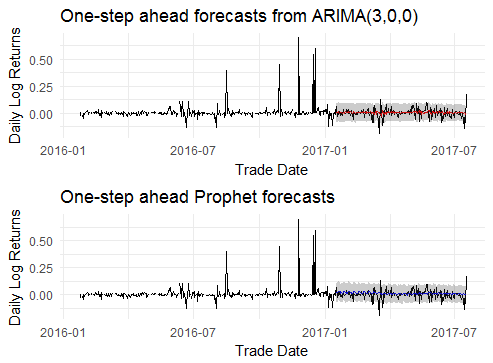
\includegraphics{C:/Users/Fiona/Documents/R/UCT_hons_proj/Draft/Figures/Evaluation of Prophet and ARIMA forecasts/1-step ahead forecasts.png}
\caption{1-step ahead forecasts from the ARIMA(1,0,0) and Prophet model}
\end{figure}

Table 1 displays the MSE and the Mincer-Zarnowitz results obtained from
regressing the test set returns against the one-step ahead forecasts.
The intercept estimate is small and positive for ARIMA and Prophet, with
the intercept for ARIMA being closer to zero than Prophet. This
indicates that both models systematically underestimate the 1-step ahead
returns, with ARIMA yielding mean forecasts closer to the observed mean.
The slope estimate is negative for both models indicating that the
observed returns are actually the opposite of the suggested forecast.
The F-test for the joint hypothesis of a unity slope and zero intercept
is rejected at the 5\% significance level for both models, with the
p-value for ARIMA being much larger than Prophet. Hence the forecasts
generated by both ARIMA and Prophet are biased and/or inefficient. The
MSE produced by both models agree with the Mincer-Zarnowitz results,
with ARIMA producing a marginally smaller MSE than Prophet.

\begin{figure}[htbp]
\centering
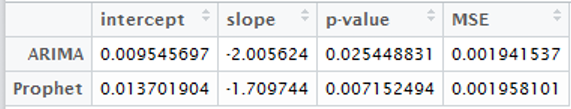
\includegraphics{C:/Users/Fiona/Documents/R/UCT_hons_proj/Draft/Figures/Evaluation of Prophet and ARIMA forecasts/Table 1.png}
\caption{Mincer-Zarnowitz results for 1-step ahead forecasts}
\end{figure}

\subsubsection{30-steps ahead Forecasts}\label{steps-ahead-forecasts}

Figure 2 illustrates the resulting 30-step ahead forecasts produced from
fitting ARIMA and Prophet. As in the 1-step ahead case, both models fail
to capture the large movement of returns away from zero with its
forecasts lying within a band centred around zero. The 80\% uncertainty
intervals produced by both models are approximately the same width and
marginally wider than the uncertainty intervals produced by the 1-step
ahead forecasts.

\begin{figure}[htbp]
\centering
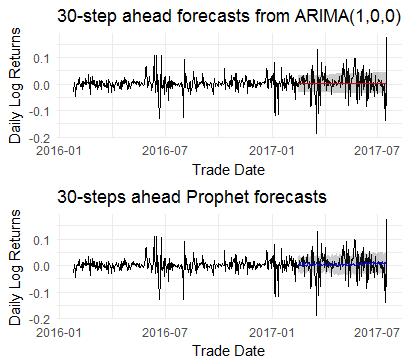
\includegraphics{C:/Users/Fiona/Documents/R/UCT_hons_proj/Draft/Figures/Evaluation of Prophet and ARIMA forecasts/30-step ahead forecasts.png}
\caption{30-step ahead forecasts from the ARIMA(1,0,0) and Prophet
model}
\end{figure}

Table 2 displays the MSE and the Mincer-Zarnowitz results obtained from
regressing the test set returns against the 30-step ahead forecasts. The
intercept estimate is small and positive for ARIMA and Prophet, with a
smaller intercept estimated for Prophet. This indicates that both models
systematically underestimate the 30-step ahead returns, with Prophet
yielding mean forecasts closer to the observed mean. The slope estimate
is large and negative for both models with the slope estimated to be as
low as -12.74 for ARIMA. This suggests that the observed returns are
actually the opposite of the proposed forecast. The F-test for the joint
hypothesis of a unity slope and zero intercept is rejected at the 5\%
significance level for Prophet only. The p-value of 0.0614 from the
joint hypothesis test is slightly significant for ARIMA. Hence the
forecasts generated by Prophet are biased and/or inefficient while the
forecasts generated by ARIMA are unbiased and/or efficient. The MSE
produced by both models agree with the Mincer-Zarnowitz results, with
ARIMA producing a marginally smaller MSE than Prophet.

\begin{figure}[htbp]
\centering
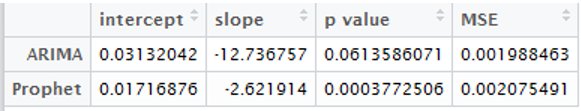
\includegraphics{C:/Users/Fiona/Documents/R/UCT_hons_proj/Draft/Figures/Evaluation of Prophet and ARIMA forecasts/Table 2.png}
\caption{Mincer-Zarnowitz results for 30-step ahead forecasts}
\end{figure}

\subsubsection{90-steps ahead Forecasts}\label{steps-ahead-forecasts-1}

Figure 3 illustrates the 90-step ahead forecasts produced by ARIMA and
Prophet. Both models fail to capture large movement of returns away from
zero as in the case of the 1-step ahead and 30-step ahead forecasts. The
80\% uncertainty intervals produced by both models are approximately the
same width and are marginally narrower than the uncertainty intervals
produced by the one-step ahead and 30-step ahead forecasts.

\begin{figure}[htbp]
\centering
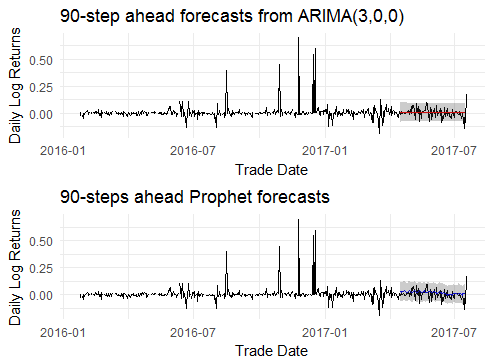
\includegraphics{C:/Users/Fiona/Documents/R/UCT_hons_proj/Draft/Figures/Evaluation of Prophet and ARIMA forecasts/90-steps ahead forecasts.png}
\caption{90-step ahead forecasts from the ARIMA(1,0,0) and Prophet
model}
\end{figure}

Table 3 presents the MSE and the Mincer-Zarnowitz results obtained from
regressing the test set returns against the 90-step ahead forecasts. The
intercept estimate is very small and positive for ARIMA and Prophet,
with a marginally smaller intercept estimated for ARIMA. This indicates
that both models systematically underestimate the 90-step ahead returns,
with ARIMA yielding mean forecasts closer to the observed mean. The
slope estimate is small and negative for both models with the slope
estimated for ARIMA lying closer to -1. This suggests that the observed
90-steps ahead returns are actually the opposite of the proposed
90-steps ahead forecasts. The F-test for the joint hypothesis of a unity
slope and zero intercept fails to be rejected at the 5\% significance
level for both ARIMA and Prophet, with the p-value from the test being
much larger for ARIMA. Hence the forecasts generated by Prophet and
ARIMA are unbiased and/or efficient. The MSE produced by both models
agree with the Mincer-Zarnowitz results, with ARIMA producing a
marginally smaller MSE than Prophet.

\begin{figure}[htbp]
\centering
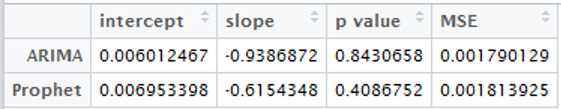
\includegraphics{C:/Users/Fiona/Documents/R/UCT_hons_proj/Draft/Figures/Evaluation of Prophet and ARIMA forecasts/Table 3.png}
\caption{Mincer-Zarnowitz results for 90-step ahead forecasts}
\end{figure}

\subsubsection{Comparison over varying forecast
horizons}\label{comparison-over-varying-forecast-horizons}

Table 4 and 5 compares the p-values obtained from the Mincer-Zarnowitz
tests and the MSE of the forecasts produced by ARIMA and Prophet over
the three forecast horizons. In comparing the forecasting accuracy of
the ARIMA model over the three forecast horizons, we observe that the
p-value gets more significant as the forecast horizon gets longer. This
is in contrast to the MSE of the ARIMA forecasts which is smaller at the
shortest and longest forecast horizons. In comparing the forecasting
accuracy of Prophet, we find that the p-value is more significant for
the shortest and longest forecast horizon. This agrees with the MSE of
the Prophet forecasts which is smaller at the longest and shortest
forecast horizon. Both ARIMA and Prophet generate forecasts with the
smallest MSE and the most significant p-value at the longest forecast
horizon. In comparing the forecasting accuracy of ARIMA and Prophet over
the three forecast horizons, we notice that the p-value obtained from
the Mincer-Zarnowitz results is more significant for ARIMA than Prophet
at every forecast horizon. This echoes the results obtained from the MSE
which is marginally smaller for ARIMA than Prophet over all forecast
horizons.

\begin{figure}[htbp]
\centering
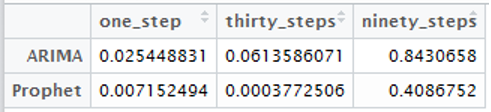
\includegraphics{C:/Users/Fiona/Documents/R/UCT_hons_proj/Draft/Figures/Evaluation of Prophet and ARIMA forecasts/Table 4.png}
\caption{Mincer-Zarnowitz results for all forecast horizons}
\end{figure}

\begin{figure}[htbp]
\centering
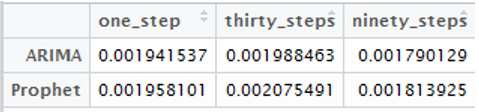
\includegraphics{C:/Users/Fiona/Documents/R/UCT_hons_proj/Draft/Figures/Evaluation of Prophet and ARIMA forecasts/Table 5.png}
\caption{MSE for all forecast horizons}
\end{figure}

\subsection{Evaluation on data with missing values and outliers
present}\label{evaluation-on-data-with-missing-values-and-outliers-present}

By following the Box-Jenkins methodology for selection of an ARIMA
model, an ARIMA(3,0,0) was employed to fit the training set which
included missing values and outliers. Although the ARIMA(0,0,3) had a
slightly smaller AIC, a decision was made to use the ARIMA(3,0,0)
instead so that a rolling window forecast may be used. Analysis of the
AR parameters indicate that they are statistically significant in the
explanation of the movement of BTC/ZAR. The Prophet model fitted to the
training set included a linear trend and weekly seasonality. All other
parameters were set to Prophet's default values as described in section
\ref{Semi-Automatic Selection}. The automatic-selection procedure for
Prophet and ARIMA selected the same models as those chosen manually.

\subsubsection{1-step ahead Forecasts}\label{step-ahead-forecasts-1}

Table 6 shows the MSE of the forecasts generated by ARIMA and Prophet
and the Mincer-Zarnowitz results obtained from regressing the test set
returns against the 1-step ahead returns forecasted. We observe that a
positive intercept is estimated in the case of ARIMA and Prophet,
indicating that both models systematically underestimate the 1-step
ahead returns. The intercept estimated for ARIMA is smaller than
Prophet, indicating that the mean forecasted returns yielded by ARIMA is
closer to the mean observed returns. The intercept estimates of 0.011895
and 0.014802 for ARIMA and Prophet respectively are larger than the
intercept estimates of 0.009546 and 0.013702, which was based on the
``clean'' dataset. This suggests that both models systematically
underestimates the returns more when there are missing values and
outliers present in the data.

We also observe that the slope estimate is small and negative for both
models with the slope estimated for ARIMA lying closer to -1. This
suggests that the observed 1-step ahead returns are actually the
opposite of the proposed 1-step ahead forecasts. The slope estimates of
-0.883228 and -0.676132 for ARIMA and Prophet respectively are less
steep than the slope estimates of -2.005624 and -1.709744, which was
based on the evaluation of data that had no values missing or outliers
present.

\begin{figure}[htbp]
\centering
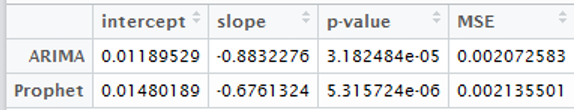
\includegraphics{C:/Users/Fiona/Documents/R/UCT_hons_proj/Draft/Figures/Evaluation of Prophet and ARIMA forecasts/Table 6.png}
\caption{Mincer-Zarnowitz results for 1-step ahead forecasts}
\end{figure}

The p-values obtained from the F-test for the joint hypothesis of a
unity slope and zero intercept is approximately zero for ARIMA and
Prophet, with the p-value for Prophet lying closer to zero than ARIMA.
The null hypothesis is thus rejected at the 1\% significance level,
indicating that the forecasts generated by Prophet and ARIMA are biased
and/or inefficient. The MSE produced by both models agree with the
Mincer-Zarnowitz results, with ARIMA producing a marginally smaller MSE
than Prophet. The results obtained from evaluating the forecasting
accuracy of ARIMA and Prophet based on the ``clean'' dataset show
similar findings, however led to a smaller MSE of 0.001942 and 0.001958
and a more significant p-value of 0.025449 and 0.007152 for ARIMA and
Prophet respectively.

\subsubsection{30-steps ahead Forecasts}\label{steps-ahead-forecasts-2}

Table 7 shows the MSE of the forecasts produced by ARIMA and Prophet and
the Mincer-Zarnowitz results obtained from regressing the test set
returns against the 30-step ahead returns forecasted. We observe that a
positive intercept is estimated in the case of ARIMA and Prophet,
indicating that both models systematically underestimate the 30-step
ahead returns. The intercept estimated for ARIMA is larger than Prophet,
indicating that the mean forecasted returns yielded by Prophet is closer
to the mean observed returns. The intercept estimate of 0.11414 for
ARIMA is larger than the estimate of 0.031320 which was based on the
evaluation of the ``clean'' dataset. This suggests that the ARIMA model
underestimates the returns more when there are missing values and
outliers present in the data. The intercept estimate of 0.014396 for
Prophet is less than the estimate of 0.017169 which was based on the
evaluation of data that had no values missing or outliers present. This
suggests that Prophet underestimates the returns less when there are
missing values and outliers present in the data.

\begin{figure}[htbp]
\centering
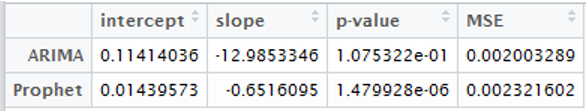
\includegraphics{C:/Users/Fiona/Documents/R/UCT_hons_proj/Draft/Figures/Evaluation of Prophet and ARIMA forecasts/Table 7.png}
\caption{Mincer-Zarnowitz results for 30-step ahead forecasts}
\end{figure}

We also observe that the slope estimate is large and negative for ARIMA
and small and negative for Prophet. This suggests that the observed
30-step ahead returns are actually the opposite of the proposed 30-step
ahead forecasts. The slope estimate of -12.985335 for ARIMA is more
steep than the slope estimate of -12.736757 which was based on the
evaluation of data that had no values missing or outliers present. This
suggests that the efficiency of the forecasted returns deteriorates when
there are missing values and outliers present in the data. The slope
estimate of -0.65161 for Prophet is less steep than the estimate
-2.621914, which was based on the evaluation of data that had no values
missing or outliers present. This suggests that the efficiency of the
forecasted returns improve when there are missing values and outliers
present in the data.

The p-value obtained from the F-test for the joint hypothesis of a unity
slope and zero intercept is approximately zero for Prophet. The null
hypothesis is thus rejected at the 1\% significance level, indicating
that the 30-step ahead forecasts generated by Prophet are biased and/or
inefficient. The p-value of 0.107532 for ARIMA is significant at the 5\%
level, suggesting at the 30-step ahead forecasts produced by ARIMA are
unbiased and/or efficient. MSE produced by both models agree with the
Mincer-Zarnowitz results, with ARIMA producing a smaller MSE than
Prophet. The results obtained from evaluating the forecasting accuracy
of ARIMA and Prophet based on the ``clean'' dataset, led to a more
significant p-value of 0.000377 for Prophet only, and a smaller MSE of
0.001988 and 0.002075 for ARIMA and Prophet respectively.

\subsubsection{90-steps ahead Forecasts}\label{steps-ahead-forecasts-3}

Table 8 shows the MSE of the forecasts produced by ARIMA and Prophet and
the Mincer-Zarnowitz results obtained from regressing the test set
returns against the 90-step ahead returns forecasted. We observe that a
negative intercept is estimated in the case of ARIMA and Prophet,
indicating that both models systematically overestimate the 90-step
ahead returns. The intercept estimated for Prophet lies closer to zero,
indicating that the mean forecasted returns yielded by Prophet is closer
to the mean observed returns. This is in contrast to the positive
intercepts that were estimated based on the data that had no values
missing or outliers present.

We also observe that the slope estimate is large and positive for ARIMA
however small and positive for Prophet. This is in contrast to the small
and negative slope estimates which were based on the evaluation of data
that had no values missing or outliers present.

\begin{figure}[htbp]
\centering
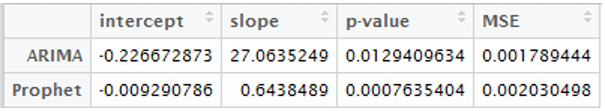
\includegraphics{C:/Users/Fiona/Documents/R/UCT_hons_proj/Draft/Figures/Evaluation of Prophet and ARIMA forecasts/Table 8.png}
\caption{Mincer-Zarnowitz results for 90-step ahead forecasts}
\end{figure}

The p-values obtained from the F-test for the joint hypothesis of a
unity slope and zero intercept are insignificant for ARIMA and Prophet,
with the p-value for Prophet lying close to zero. The null hypothesis is
thus rejected at the 5\% significance level, indicating that the
90-steps ahead forecasts generated by Prophet and ARIMA are biased
and/or inefficient. The MSE produced by both models agree with the
Mincer-Zarnowitz results, with ARIMA producing a marginally smaller MSE
than Prophet. The results obtained from evaluating the forecasting
accuracy of ARIMA and Prophet based on data which had no missing values
or outliers present contrasts these findings, with a p-value of 0.843066
and 0.408675 for ARIMA and Prophet respectively.

\subsubsection{Comparison over varying forecast
horizons}\label{comparison-over-varying-forecast-horizons-1}

Table 9 and 10 compares the p-values obtained from the Mincer-Zarnowitz
tests and the MSE of the forecasts produced by ARIMA and Prophet over
the three forecast horizons. In comparing the forecasting accuracy of
the ARIMA model over the three forecast horizons, we observe that the
p-value is more significant at the longer forecast horizons. This agrees
with the MSE of the ARIMA forecasts which is smaller at the longer
forecast horizons. In comparing the forecasting accuracy of Prophet, we
find that the p-value is more significant for the longest forecast
horizon. This agrees with the MSE of the Prophet forecasts which is
smaller at the longest forecast horizon.

\begin{figure}[htbp]
\centering
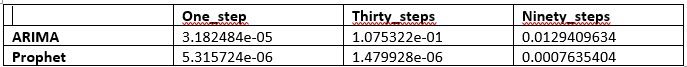
\includegraphics{C:/Users/Fiona/Documents/R/UCT_hons_proj/Draft/Figures/Evaluation of Prophet and ARIMA forecasts/Table 9.png}
\caption{Mincer-Zarnowitz results for all forecast horizons}
\end{figure}

\begin{figure}[htbp]
\centering
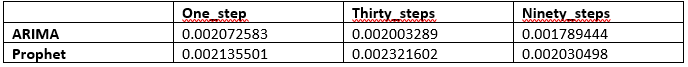
\includegraphics{C:/Users/Fiona/Documents/R/UCT_hons_proj/Draft/Figures/Evaluation of Prophet and ARIMA forecasts/Table 10.png}
\caption{MSE for all forecast horizons}
\end{figure}

In comparing the forecasting accuracy of ARIMA and Prophet over the
three forecast horizons, we notice that the p-value obtained from the
Mincer-Zarnowitz results is more significant for ARIMA than Prophet at
every forecast horizon. This echoes the results obtained from the MSE
which is marginally smaller for ARIMA than Prophet over all forecast
horizons.

\section{\texorpdfstring{Discussion and Conclusions
\label{Discussion and Conclusions}}{Discussion and Conclusions }}\label{discussion-and-conclusions}

The results show a clear difference in the effect of the forecast
horizon in the case of the clean data. The results based on the MSE and
the p-value obtained from the Mincer-Zarnowitz test surprisingly show
that the ARIMA model produces superior forecasts of the returns at the
longest forecast horizon. Similarly, Prophet produces superior forecasts
of the returns at the longest forecast horizon. We notice that although
the ARIMA model outperforms Prophet at every forecast horizon, the
difference between the MSE's of the forecasts generated by both models
is insignificant. Furthermore, the Mincer-Zarnowitz p-values for both
models are significant at the same forecast horizons, suggesting that
the efficiency and biasness of the return forecasts yielded by ARIMA and
Prophet are synchronized at each forecast horizon. If a small amount of
predictive accuracy is willing to be sacrificed by the analyst in the
forecasting of BTC/ZAR, it might be useful to employ Prophet instead of
ARIMA. This would enable traders with expert knowledge about Bitcoin,
however no statistical knowledge about forecasting models, to
incorporate their domain knowledge into the Prophet model through its
intuitively adjustable parameters. Furthermore, as more information
about events that may affect the price of Bitcoin becomes available, it
may be included in the model and could potentially change the predictive
accuracy of Prophet.

The results based on the unclean data show that both ARIMA and Prophet
are sensitive to the presence of outliers and missing values in addition
to the forecast horizon. We observe that Prophet yields superior
forecasts at the longest forecast horizon. Although the MSE suggests
that the ARIMA model produces forecasts with minimal error at the
longest forecast horizon, analysis of the p-value indicates that the
forecasts are efficient and/or unbiased at 30-steps ahead only. It is
evident that Prophet produces inferior results in comparison to the
ARIMA model over all forecast horizons. This is unexpected as Prophet is
said to be robust to the presence of outliers and missing values in the
data, without the need for interpolation. We also notice that the
forecasts produced by both models deteriorates when there are missing
values and outliers present in the data, with the only efficient and/or
unbiased forecasts yielded by the ARIMA model at a forecast horizon of
30 days.

The limitation of this study is that it looks specifically at BTC/ZAR.
Different results may emerge for fiat currencies or the exchange rate
between Bitcoin with other currencies. Hence caution should be exercised
when generalising these results to other exchange rates. As a point of
further research, more complex techniques such as neural networks could
be used as a benchmark for comparison when evaluating the forecasts
produced by Prophet.

\newpage

\section*{References}\label{references}
\addcontentsline{toc}{section}{References}

\hypertarget{refs}{}
\hypertarget{ref-abu1996}{}
Abu-Mostafa, Yaser S, and Amir F Atiya. 1996. ``Introduction to
Financial Forecasting.'' \emph{Applied Intelligence} 6 (3). Springer:
205--13.

\hypertarget{ref-anastasakis2009}{}
Anastasakis, Leonidas, and Neil Mort. 2009. ``Exchange Rate Forecasting
Using a Combined Parametric and Nonparametric Self-Organising Modelling
Approach.'' \emph{Expert Systems with Applications} 36 (10). Elsevier:
12001--11.

\hypertarget{ref-castillo2002}{}
Castillo, Oscar, and Patricia Melin. 2002. ``Hybrid Intelligent Systems
for Time Series Prediction Using Neural Networks, Fuzzy Logic, and
Fractal Theory.'' \emph{IEEE Transactions on Neural Networks} 13 (6).
IEEE: 1395--1408.

\hypertarget{ref-cheung1993}{}
Cheung, Yin-Wong. 1993. ``Long Memory in Foreign-Exchange Rates.''
\emph{Journal of Business \& Economic Statistics} 11 (1). Taylor \&
Francis: 93--101.

\hypertarget{ref-etuk2013}{}
Etuk, Ette Harrison, Dagogo SA Wokoma, and Imoh Udo Moffat. 2013.
``Additive Sarima Modelling of Monthly Nigerian Naira-Cfa Franc Exchange
Rates.'' \emph{European Journal of Statistics and Probability} 1 (1):
1--12.

\hypertarget{ref-fahimifard2009}{}
Fahimifard, SM, Masuod Homayounifar, M Sabouhi, and AR Moghaddamnia.
2009. ``Comparison of Anfis, Ann, Garch and Arima Techniques to Exchange
Rate Forecasting.'' \emph{Journal of Applied Sciences} 9 (20): 3641--51.

\hypertarget{ref-spyros1997}{}
Hibon, Michael, and Spyros Makridakis. 1997. ``ARMA Models and the
Box--Jenkins Methodology.'' John Wiley \& Sons, Ltd.

\hypertarget{ref-ince2006}{}
Ince, Huseyin, and Theodore B Trafalis. 2006. ``A Hybrid Model for
Exchange Rate Prediction.'' \emph{Decision Support Systems} 42 (2).
Elsevier: 1054--62.

\hypertarget{ref-kamruzzaman2003}{}
Kamruzzaman, Joarder, and Ruhul A Sarker. 2003. ``Forecasting of
Currency Exchange Rates Using Ann: A Case Study.'' In \emph{Neural
Networks and Signal Processing, 2003. Proceedings of the 2003
International Conference on}, 1:793--97. IEEE.

\hypertarget{ref-khashei2011}{}
Khashei, Mehdi, and Hehdi Bijari. 2011. ``Exchange Rate Forecasting
Better with Hybrid Artificial Neural Networks Models.'' \emph{Journal of
Mathematical and Computational Science} 1 (1). Science \& Knowledge
Publishing Corporation Limited (SCIK): 103.

\hypertarget{ref-khashei2009}{}
Khashei, Mehdi, Mehdi Bijari, and Gholam Ali Raissi Ardali. 2009.
``Improvement of Auto-Regressive Integrated Moving Average Models Using
Fuzzy Logic and Artificial Neural Networks (Anns).''
\emph{Neurocomputing} 72 (4). Elsevier: 956--67.

\hypertarget{ref-khashei2012}{}
---------. 2012. ``Hybridization of Autoregressive Integrated Moving
Average (Arima) with Probabilistic Neural Networks (Pnns).''
\emph{Computers \& Industrial Engineering} 63 (1). Elsevier: 37--45.

\hypertarget{ref-lin2012}{}
Lin, Chiun-Sin, Sheng-Hsiung Chiu, and Tzu-Yu Lin. 2012. ``Empirical
Mode Decomposition--based Least Squares Support Vector Regression for
Foreign Exchange Rate Forecasting.'' \emph{Economic Modelling} 29 (6).
Elsevier: 2583--90.

\hypertarget{ref-mincer1969}{}
Mincer, Jacob A, and Victor Zarnowitz. 1969. ``The Evaluation of
Economic Forecasts.'' In \emph{Economic Forecasts and Expectations:
Analysis of Forecasting Behavior and Performance}, 3--46. NBER.

\hypertarget{ref-nwankwo2014}{}
Nwankwo, Steve C. 2014. ``Autoregressive Integrated Moving Average
(Arima) Model for Exchange Rate (Naira to Dollar).'' \emph{Academic
Journal of Interdisciplinary Studies} 3 (4): 429.

\hypertarget{ref-santos2007}{}
Santos, André Alves Portela, Newton Carneiro Affonso da Costa, and
Leandro dos Santos Coelho. 2007. ``Computational Intelligence Approaches
and Linear Models in Case Studies of Forecasting Exchange Rates.''
\emph{Expert Systems with Applications} 33 (4). Elsevier: 816--23.

\hypertarget{ref-taylor2017}{}
Taylor, Sean J, and Benjamin Letham. 2017. ``Forecasting at Scale.''

\hypertarget{ref-tseng2001}{}
Tseng, Fang-Mei, Gwo-Hshiung Tzeng, Hsiao-Cheng Yu, and Benjamin JC
Yuan. 2001. ``Fuzzy Arima Model for Forecasting the Foreign Exchange
Market.'' \emph{Fuzzy Sets and Systems} 118 (1). Elsevier: 9--19.

\hypertarget{ref-zhang1998}{}
Zhang, Gioqinang, and Michael Y Hu. 1998. ``Neural Network Forecasting
of the British Pound/Us Dollar Exchange Rate.'' \emph{Omega} 26 (4).
Elsevier: 495--506.

\newpage
\renewcommand{\baselinestretch}{1}
\nocite{*}
\bibliography{}

\end{document}
